\documentclass{beamer}
\usetheme{Warsaw}
\usepackage{ragged2e}
\usepackage{multimedia}
\usepackage{polski}
\usepackage[utf8]{inputenc}
\usecolortheme{beaver}
\title[]
{Algorytmy filtrowania w programowaniu ograniczeń}
\author[]
{
    autor: Tomasz Kulik \\
    promotor: dr Przemysław Kobylański
}
\institute[Politechnika Wrocławska]
{
  Wydział Podstawowych Problemów Techniki \\
  Politechnika Wrocławska \\
  Polska
}
\date[2019]
{2019}
\subject{Informatyka (spec. algorytmika)}



\begin{document}
    \begin{frame}
        \titlepage
    \end{frame}


    \section{Wstęp}
    \begin{frame}
    	\frametitle{Zakres pracy}
        \begin{itemize}
            \item Wprowadzenie do programowania z ograniczeniami
            \item Omówienie podstawowych pojęć związanych z językami regularnymi
            \item Wprowadzenie nowego algorytmu propagującego ograniczenia
            \item Przedstawienie wyników pracy
        \end{itemize}
    \end{frame}
    \begin{frame}
    	\frametitle{Narzędzia}
        \begin{itemize}
            \item C++11 z wykorzystaniem biblioteki standardowej
            \item IBM ILOG CPLEX CP Optimizer
        \end{itemize}
    \end{frame}


    \section{Programowanie z ograniczeniami}
    \begin{frame}
        \frametitle{Programowanie z ograniczeniami}
        Paradygmat pozwalający na modelowanie:
        \begin{itemize}
            \item systemów wspomagających podejmowanie decyzji
            \item problemów kombinatorycznych
            \item problemów planistycznych (logistycznych)
            \item problemów optymalizacyjnych
        \end{itemize}
    \end{frame}


    \begin{frame}
        \frametitle{Problem spełnienia ograniczeń}
        Formalnie problem spełnienia ograniczeń $P$ to trójka $(X, D, C)$, gdzie:
        \begin{itemize}
            \item $X$ - n-elementowa krotka $(X_1, X_2, ... , X_n)$ zmiennych,
            \item $D$ - n-elementowa krotka $(D_1, D_2, ... , D_n)$ zbiorów stanowiących dziedziny odpowiadających zmiennych z
                        krotki X, tj. $X_i \in D_i$,
            \item $C$ - t-elementowa krotka $(C_1, C_2, ... , C_t)$ ograniczeń narzuconych na zmienne z krotki $X$.
        \end{itemize}
    \end{frame}
    \begin{frame}
    	\frametitle{Przykład}
        \begin{example}
            \textbf{Problem spełnienia ograniczeń:}
            \begin{equation}
                \left\{
                    \begin{aligned}
                        X &= (A, B, C), \\
                        D &= (\{2,3\}, \{3,4\}, \{8,16,32\})
                    \end{aligned}
                \right.
            \end{equation}
            Ograniczenia:
            \begin{equation}
                \left\{
                    \begin{aligned}
                        3A &> C \\
                        3B &> C \\
                        A &\neq B,
                    \end{aligned}
                \right.
            \end{equation}
            Rozwiązanie: $(A=3, B=4, C=8)$.
            \end{example}
    \end{frame}
    \begin{frame}
        \frametitle{Przeszukiwanie, propagacja ograniczeń}
        Algorytmy poszukujące rozwiązań problemów programowania z ograniczeniami
        posługują się dwoma podstawowymi technikami:
        \begin{itemize}
            \item Przeszukiwanie drzewa rozwiązań
            \item Iteracyjna propagacja ograniczeń na dziedzinach zmiennych
        \end{itemize}
    \end{frame}
    \begin{frame}
        \frametitle{Ograniczenia globalne}
        \begin{itemize}
            \item Globalne ograniczenia są to takie ograniczenia, które wiążą ze sobą dowolną liczbę
                  zmiennych.
            \item Globalne ograniczenia pozwalają na wprowadzenie skuteczniejszych metod
                  propagowania ograniczeń dla konkretnych problemów
            \item Sztandarowy przykład: \bf{AllDifferent($X_1, X_2, ... , X_k$)}
        \end{itemize}
    \end{frame}


    \section{Języki regularne}
    \begin{frame}
    	\frametitle{Następny rozdział}
        \tableofcontents[currentsection]
    \end{frame}
    \begin{frame}
        \frametitle{Formalna definicja}
        Języki rozstrzygalne przez automaty skończone. \\
        Każdy automat skończony można przedstawić w formie gramatyki regularnej. \\
        Dwa rodzaje automatów skończonych:
        \begin{itemize}
            \item Deterministyczne Automaty Skończone (\textit{ang. DFA})
            \item Niedeterministyczne Automaty Skończone (\textit{ang. NFA})
        \end{itemize}
        Każdemu niedeterministycznemu automatowi skończonemu odpowiada deterministyczny automat
        skończony akceptujący dokładnie te same słowa. Relacja działa również w przeciwną stronę.
    \end{frame}
    \begin{frame}
        \frametitle{Wyrażenia regularne}
        Wyrażenia regularne powstałe przy użyciu poniższych operatorów opisują gramatyki regularne:
        \begin{itemize}
            \item Konkatenacja (\textit{$AB$})
            \item Alternatywa (\textit{$A|B$})
            \item Domknięcie Kleene'ego (\textit{$A^*$})
        \end{itemize}
    \end{frame}


    \section{Algorytm filtrujący}
    \begin{frame}
		\frametitle{Następny rozdział}
        \tableofcontents[currentsection]
    \end{frame}
    \begin{frame}
        \frametitle{Metoda Thompsona}
        Metoda pozwalająca na translację wyrażeń regularnych na automaty $NFA$.
        \begin{center}
            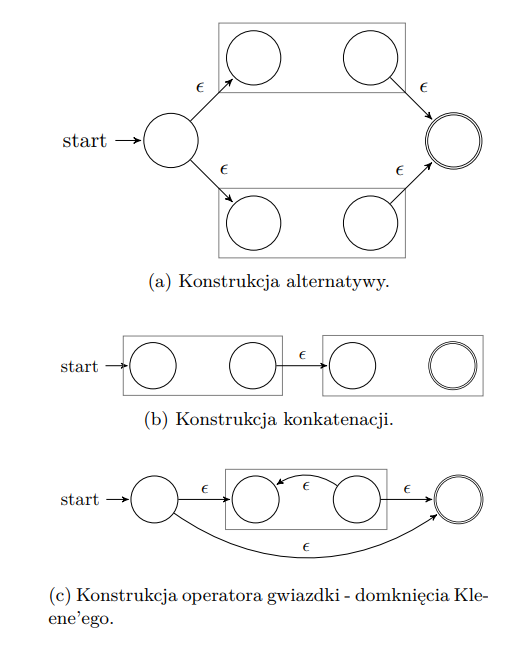
\includegraphics[width=0.45\textwidth]{thompson.png}
        \end{center}
    \end{frame}
    \begin{frame}
        \frametitle{Metoda RegexFiltering}
        \begin{center}
            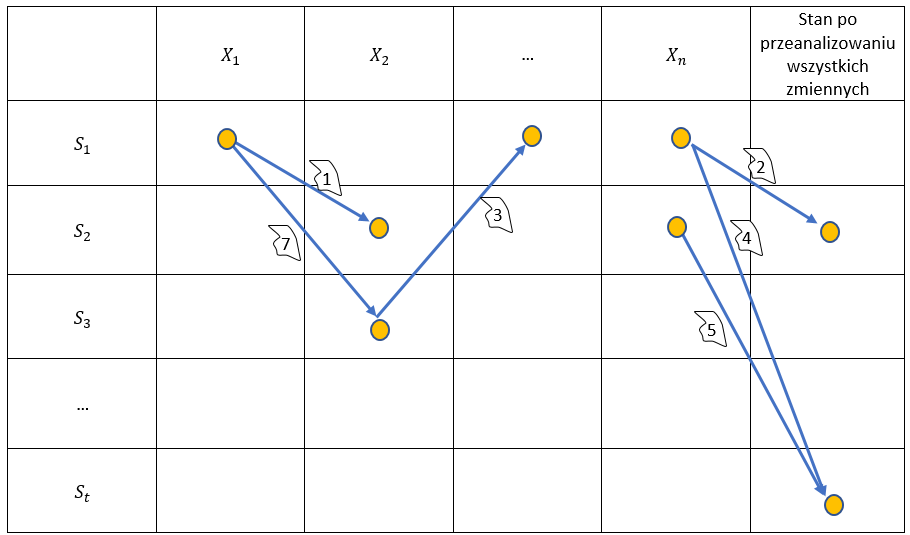
\includegraphics[width=0.7\textwidth]{regex_filtering.png}
        \end{center}
    \end{frame}
    \begin{frame}
        \frametitle{Metoda RegexFiltering}
        \begin{itemize}
            \item Dla każdej zmiennej stwórz pusty kontener
            \item Na podstawie struktury wypełnionej ścieżkami pomiędzy stanami automatów
                należy przejść przez wszystkie ścieżki wychodzące ze stanu akceptującego
                (zaczynając w stanie akceptującym od ostatniej zmiennej)
            \item Przechodząc przez ścieżki należy dodawać do kontenerów każdej zmiennej
                wartości zaakceptowane przez automat.
        \end{itemize}
        Zbiór wypełnionych kontenerów stanowi nowy zbiór dziedzin dla analizowanych zmiennych.
    \end{frame}


    \section{Złożoność obliczeniowa}
    \begin{frame}
		\frametitle{Następny rozdział}
        \tableofcontents[currentsection]
    \end{frame}
    \begin{frame}
    	\frametitle{Złożoność Obliczeniowa}
        \begin{itemize}
            \item Złożoność czasowa wynosi $O(nk^2)$
            \item Złożoność pamięciowa wynosi $O(nk)$
        \end{itemize}
        $n$ - liczba zmiennych w wektorze wejściowym \\
        $k$ - liczba stanów automatu wygenerowanego na podstawie wyrażenia regularnego
    \end{frame}
    \begin{frame}
        \frametitle{Eksperymenty}
        \begin{center}
            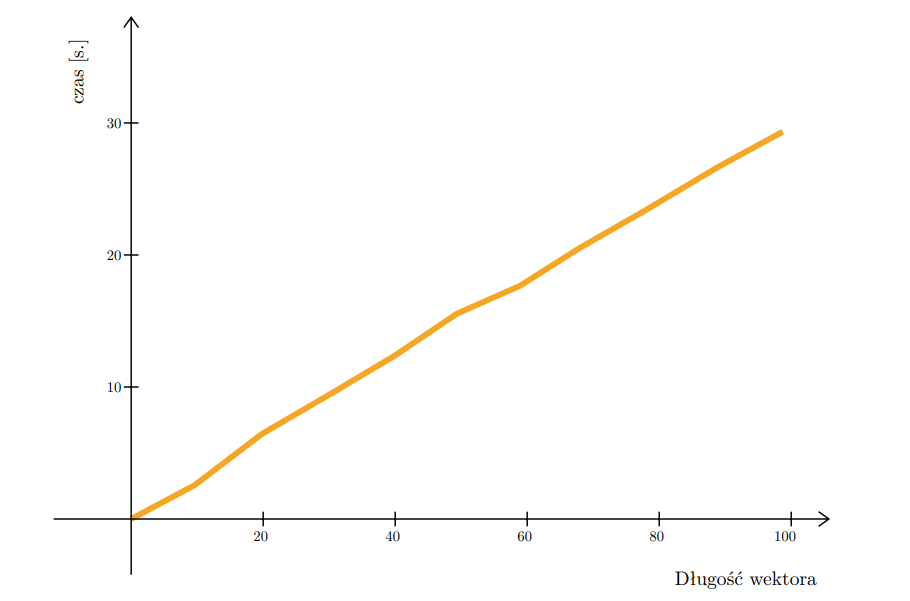
\includegraphics[width=0.5\textwidth]{vec_len.png}
            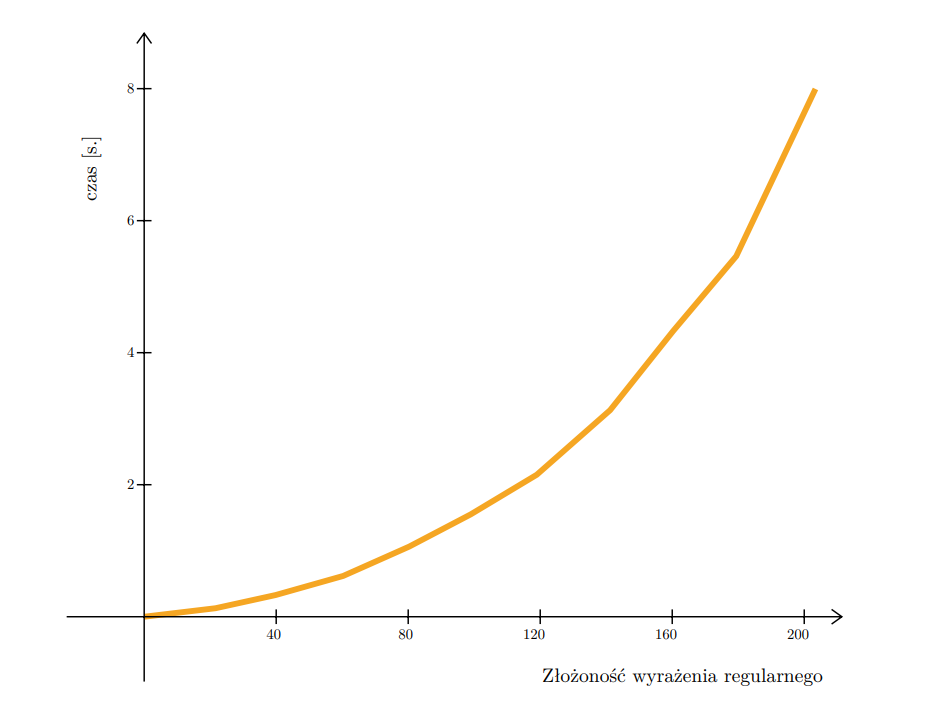
\includegraphics[width=0.5\textwidth]{vec_complex.png}
        \end{center}
    \end{frame}


    \section{Zastosowanie}
    \begin{frame}
		\frametitle{Następny rozdział}
        \tableofcontents[currentsection]
    \end{frame}
    
    \begin{frame}
    	\frametitle{Rozmieszczanie odcinków}
        \begin{itemize}
            \item Rozmieszczanie odcinków w wektorze zmiennych
            \item Łączenie z innymi ograniczeniami (np. w celu narzucania zadanej liczby przegięć funkcji)
            \item Rozwiązywanie zagadek typu \textit{Nonograms}
        \end{itemize}
    \end{frame}

    \begin{frame}
        \frametitle{Przykład nonogramu}
        \begin{center}
            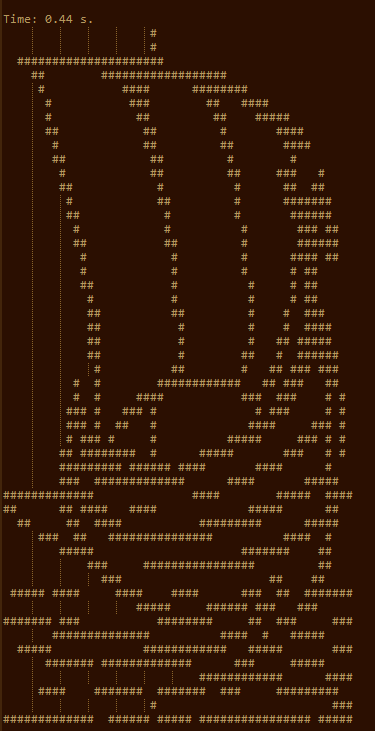
\includegraphics[width=0.4\textwidth]{drakkar.png}
        \end{center}
    \end{frame}
    \begin{frame}
        \frametitle{Porównanie z SWI-Prolog}
        \begin{center}
            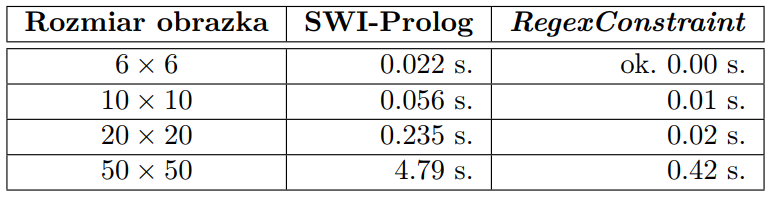
\includegraphics[width=0.6\textwidth]{time_results.png}
        \end{center}
    \end{frame}


    \section{Podsumowanie}
    \begin{frame}
		\frametitle{Następny rozdział}
        \tableofcontents[currentsection]
    \end{frame}
    \begin{frame}
    	\frametitle{Dalszy rozwój}
        \begin{itemize}
            \item Wprowadzenie bogatszej gramatyki wyrażeń regularnych
            \item Rozszerzenie algorytmu o obsługę liczników (możliwość modelowania szerszej klasy problemów)
        \end{itemize}
    \end{frame}
    \begin{frame}
        \frametitle{Dziękuję za uwagę!}
    \end{frame}


\end{document}
